%%%%%%%%%%%%%%%%%%%%%%%%%%%%%%%%%%%%%%%%%%%%%%%%%%%%%%%%%%%%%%%%%%%
%% chapter1.tex
%% NOVA thesis document file
%%
%% Chapter with introduction
%%%%%%%%%%%%%%%%%%%%%%%%%%%%%%%%%%%%%%%%%%%%%%%%%%%%%%%%%%%%%%%%%%%

\typeout{NT FILE chapter3.tex}%

\chapter{SDR Control}
\label{cha:sdr-control}

\prependtographicspath{{\DIRFIGURES/Covers/}}

This chapter describes the \gls{sdr-control-system} used in this internship.
The \gls{sdr-control-system} is responsible for managing the communication
between the \gls{SDR} hardware and the software applications that utilize it.
It provides an interface for configuring the \gls{SDR} parameters, such as
Frequency, \gls{RF}-control, and Sampling Rate, as well as handling data
transmission.

\section{Objective and Motivation}
\label{sec:sdr-objective-and-motivation}

One of the main problems in this internship, whilst developing the
\gls{sdr-control-system}, was the lack of an easy to use interface. Whilst
\gls{DTAPI}, the \gls{sdr-control-system} library used in this internship,
provides a powerful set of instructions to control the \gls{SDR} hardware, its
interface is not user-friendly, due to its requirement to chain calls
correctly, the heavy use of macros, manual device state management and it does
not offer a clean way to manage the \gls{SDR} parameters. To address this
issue, the \gls{sdr-control-system} was designed to provide a more intuitive
and user-friendly interface for managing parameters and operations, either by
providing easy to use abstractions to transmit signals, or by providing
synchronization mechanisms between devices.

\section{Design and Implementation}
\label{sec:sdr-design-and-implementation}

The \gls{sdr-control-system} was implemented using a modular approach, with
separate components responsible for device management, signal playback,
synchronization, etc.. A design goal of the internship was to integrate this
system with other components, that will not be described here due to the scope
of this report and their proprietary nature, to provide a complete solution for
\gls{GNSS} signal generation. Thus the system was designed with a client server
architecture, where the control system acts as a server that listens for
commands from client applications and executes them accordingly. The
communication between the server and client is handled through a \gls{gRPC}
interface, which allows for remote procedure calls and provides a structured
way to manage the interactions between the different components of the system.
To note that an unintended, but useful nonetheless, feature of this
architecture is that it allows users to create \textit{bash} scripts that can
interact with the system through the client executable, which can be useful for
quick testing and automation purposes.

% Design choices
It is also relevant to note some of the design choices made during the
implementation of the \gls{sdr-control-system}. The most impactful one is the
use of \gls{gRPC} for three main reasons: it has proven itself in terms of
reliability and performance, it provides a clear and strongly typed interface
for communication between the server and client, and allows for reflection, the
latter being one of the most useful features during development, as it not only
allows for easy debugging and testing, easy configuration parsing, but also
allows the user to easily discover the available commands and their parameters,
which is especially useful for users that are not familiar with the system.
Another quite relevant, but not as impactful design choice was the use of
errors as values instead of the traditional approach of using exceptions. This
aided not only in making a more concise interface, but also avoids some of the
performance pitfalls of exceptions. Another quite impactful decision that
deviates from the norm was the build system used, usually the default
buildsystem is CMake\footnote{CMake is a powerful yet complex build
  system.\cite{cmake}}, though XMake was chosen, XMake is a more modern and
user-friendly build system, which allows for a more concise and easier to
maintain build configuration, as well as an extremely easy to use package
manager and faster build times, when compared to CMake and Ninja\footnote{Ninja
  is a small build system with a focus on speed.\cite{ninja-build}}, due to its
caching mechanism\cite{xmake}\cite{xmake-cache}.

The design described above is the result of the third iteration of the
\gls{sdr-control-system}. The two earlier attempts, and the reasoning behind
their abandonment, are documented in
\autoref{sec:design-patterns:sdr-iterations}, as several of the design choices
discussed in this chapter were directly informed by that history.

% Limitations

Some of the limitations of the current implementation of the
\gls{sdr-control-system} are related to the client server architecture. One of
the main limitations is that it introduces some latency in the communication
between the server and client, due to a client being created on binary boot,
which can be an issue for real-time applications, to note that this is only a
problem due to the client being a \gls{CLI}. It is worth noting, however, that
this latency concern was not actually encountered in practice, as discussed in
\autoref{sec:integration}, the gRPC layer was ultimately deemed unnecessary for
the integration with GMV's proprietary systems, which instead linked the
\texttt{app} component directly in-process. Additionally, whilst on purpose,
the coupling between the system and \gls{gRPC} is notable. Another limitation
is that the current implementation does not support all the features of the
\gls{SDR} hardware, though this cant really be considered a problem as those
features are outside the scope of this internship and can be easily added in
the future if needed.

\section{IQ Signal Generation}
\label{sec:iq-signal-generation}

Whilst not the main focus of this internship, the \gls{sdr-control-system} is
designed to integrate with a \gls{GNSS} signal generation system, which is
responsible for generating the actual \gls{I/Q} samples that are transmitted
through the \gls{SDR} hardware. Since such component was still unfinised a
simplified model of the signal generation was implemented, which allows for the
generation of single tone signals with configurable parameters, such as
frequency, amplitude, phase, Doppler shift and code delay. This simplified
model was sufficient for the purpose of testing the \gls{sdr-control-system}
and its integration with the \gls{SDR} hardware, but it is expected that a more
sophisticated signal generation system will be integrated in the future.

\subsection{In-phase and Quadrature Components}

A signal intended for transmission is represented in baseband by two orthogonal
components, the in-phase component, $I(t)$, and the quadrature component,
$Q(t)$. Together they describe a complex baseband signal $s(t) = I(t) + jQ(t)$,
which is later mixed up to the desired carrier frequency by the \gls{SDR}
hardware. For a single tone, the two components are given by

\begin{equation}
  I(t) = A\cos\left(2\pi f t + \varphi\right), \qquad
  Q(t) = A\sin\left(2\pi f t + \varphi\right),
  \label{eq:iq-components}
\end{equation}

\noindent where $A$ is the amplitude, $f$ is the frequency, and $\varphi$ is
the phase of the signal. Figure~\ref{fig:iq-components} shows an example of
these two components plotted over time, with a $90\degree$ phase offset
between them, which is what gives the quadrature component its name.\cite{pysdrSamplingPySDR}

\begin{figure}[htbp]
  \centering
  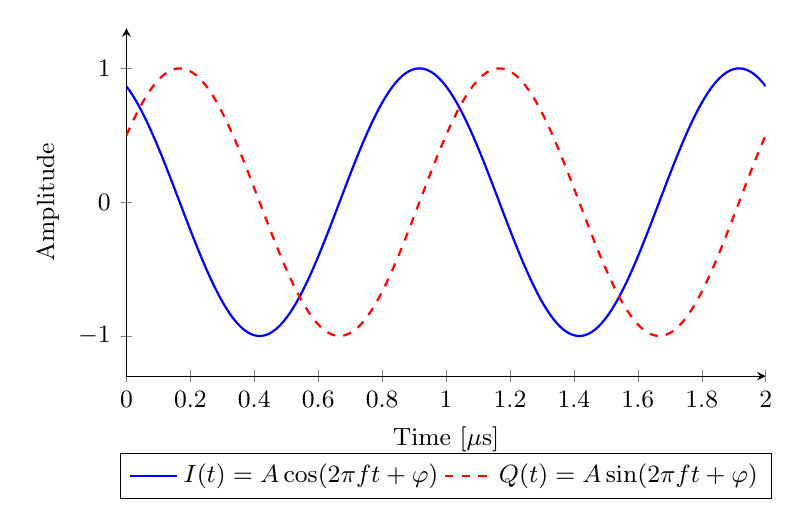
\begin{tikzpicture}
    \begin{axis}[
        width=0.8\textwidth, height=6cm,
        xlabel={Time [$\mu$s]},
        ylabel={Amplitude},
        xmin=0, xmax=2,
        ymin=-1.3, ymax=1.3,
        legend style={at={(0.5,-0.22)}, anchor=north, legend columns=2},
        axis lines=left,
        ticklabel style={font=\small},
        label style={font=\small},
        legend style={font=\small},
      ]
      \addplot[domain=0:2, samples=200, thick, blue] {cos(2*360*0.5*x + 30)};
      \addlegendentry{$I(t) = A\cos(2\pi f t + \varphi)$}
      \addplot[domain=0:2, samples=200, thick, red, dashed] {sin(2*360*0.5*x + 30)};
      \addlegendentry{$Q(t) = A\sin(2\pi f t + \varphi)$}
    \end{axis}
  \end{tikzpicture}
  \caption{In-phase and quadrature components of a single-tone baseband signal.}
  \label{fig:iq-components}
\end{figure}

Amplitude, frequency and phase are thus the three basic parameters that both
the signal generator and the \gls{sdr-control-system} expose for a given signal
channel. Amplitude controls the transmitted power level, frequency determines
the carrier offset within the channel bandwidth, and phase allows for fine
alignment between multiple signals or devices, which becomes particularly
relevant when synchronizing several \gls{SDR} channels, as mentioned in
Section~\ref{sec:sdr-functionality-and-use-cases}.

\subsection{Doppler Effect}

In the context of \gls{GNSS} signal simulation, the relative motion between a
satellite and a receiver introduces a Doppler shift on the carrier frequency.
This shift is not constant, as it depends on the relative velocity along the
line of sight between transmitter and receiver, which changes over the course
of a satellite pass. Figure~\ref{fig:doppler} illustrates a typical Doppler
profile for a satellite pass, where the shift starts positive as the satellite
approaches, crosses zero near the point of closest approach, and becomes
negative as the satellite recedes.

\begin{figure}[htbp]
  \centering
  \begin{tikzpicture}
    \begin{axis}[
        width=0.7\textwidth, height=6cm,
        xlabel={Time [s]},
        ylabel={Doppler shift $f_d$ [kHz]},
        xmin=0, xmax=10,
        axis lines=left,
        ticklabel style={font=\small},
        label style={font=\small},
      ]
      \addplot[domain=0:10, samples=100, thick, blue] {2.2 * (1 - 2/(1+exp(-1.2*(x-5))))};
    \end{axis}
  \end{tikzpicture}
  \caption{Example Doppler shift profile over the course of a satellite pass.}
  \label{fig:doppler}
\end{figure}

To support this, the signal generator allows the Doppler shift to be specified
as a parameter of the generated signal.

\subsection{Code Delay}

\gls{GNSS} signals are modulated with a pseudorandom ranging code, which the
receiver correlates against a locally generated replica to estimate the
propagation delay between satellite and receiver. This propagation delay,
referred to as the code delay $\tau$, is what ultimately allows the receiver
to compute its position, and it is usually expressed in chips of the ranging
code rather than in absolute time. As the geometric distance between satellite
and receiver changes, so does the code delay, typically increasing or
decreasing smoothly over time, as illustrated in
Figure~\ref{fig:code-delay}.

\begin{figure}[htbp]
  \centering
  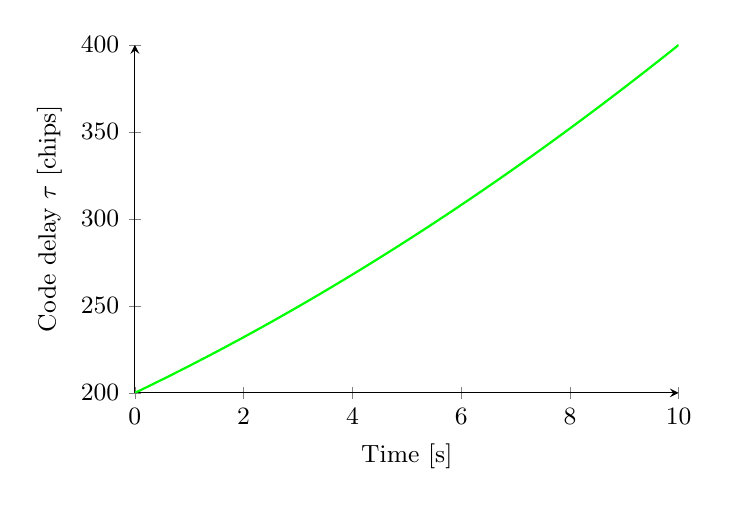
\begin{tikzpicture}
    \begin{axis}[
        width=0.7\textwidth, height=6cm,
        xlabel={Time [s]},
        ylabel={Code delay $\tau$ [chips]},
        xmin=0, xmax=10,
        axis lines=left,
        ticklabel style={font=\small},
        label style={font=\small},
      ]
      \addplot[domain=0:10, samples=100, thick, green] {200 + 15*x + 0.5*x*x};
    \end{axis}
  \end{tikzpicture}
  \caption{Example code delay evolution over time.}
  \label{fig:code-delay}
\end{figure}

Similarly to the Doppler shift, the code delay can be configured in the signal
generator as a parameter of the generated signal, allowing the simulation of
realistic satellite-to-receiver geometries without requiring an actual moving
transmitter.

\section{Architecture Diagram}
Diagram \ref{fig:sdr-control-architecture} illustrates the architecture of the
\gls{sdr-control-system}, showing the main components and their interactions.
The diagram highlights the client-server architecture, the use of \gls{gRPC}
for communication, and the integration with the \gls{DTAPI} library for
hardware control. It also includes annotations that provide additional context
and explanations for the design choices made in the implementation of the
system.

\begin{figure}[htbp]
  \centering
  \usetikzlibrary{positioning, fit, backgrounds, arrows.meta, calc}
\begin{tikzpicture}[
        % ── node styles ─────────────────────────────────────────
        comp/.style = { draw, rounded corners=3pt, minimum width=3.0cm, minimum
                height=1.5cm, text width=2.8cm, align=center, font=\small, inner sep=5pt, },
        lollipop/.style = { draw, circle, minimum size=0.32cm, inner sep=0pt,
                fill=white, }, stereo/.style = {font=\tiny\itshape, text=gray!60}, use/.style =
            {->, >=open triangle 45, dashed, thick}, realize/.style = {->, >=open triangle
                45, dashed, thick, double distance=1.2pt}, assoc/.style = {thick}, note/.style
            = { draw=gray!40, fill=yellow!8, rounded corners=2pt, font=\tiny, text
                width=2.8cm, align=left, inner sep=4pt, }, node distance = 1.4cm, ]

    % ============================================================
    % ROW 1 — CLI Client  |  Server
    % ============================================================
    \node[comp, fill=green!10, draw=green!55!black]
    (client) at (0,0)
    {\texttt{<<component>>}\\[3pt]\textbf{\gls{CLI} Client}};

    \node[comp, fill=green!10, draw=green!55!black,
        right=5.0cm of client]
    (server)
    {\texttt{<<component>>}\\[3pt]\textbf{Server}};

    % ============================================================
    % ROW 2 — Public API  |  dt\_facade  |  dt
    % ============================================================
    % Public API sits between client and server, one row below
    \node[comp, fill=blue!10, draw=blue!50,
    below=3.0cm of $(client)!0.5!(server)$]
    (pubapi)
    {\texttt{<<component>>}\\[3pt]\textbf{Public API}\\[2pt]
    {\tiny\textcolor{gray!60}{(generated by \texttt{protoc})}}};

    \node[comp, fill=blue!10, draw=blue!50,
    below=3.2cm of server]
    (dtfacade)
    {\texttt{<<component>>}\\[3pt]\textbf{dt\_facade}\\[2pt]
    {\tiny\textcolor{gray!60}{(dtapi high level wrapper)}}};

    \node[comp, fill=blue!10, draw=blue!50,
    right=2.6cm of dtfacade]
    (dt)
    {\texttt{<<component>>}\\[3pt]\textbf{dt}\\[2pt]
    {\tiny\textcolor{gray!60}{(utility library)}}};

    % ============================================================
    % ROW 3 — DTAPI
    % ============================================================
    \node[comp, fill=red!10, draw=red!45,
    below=2.8cm of dtfacade]
    (dtapi)
    {\texttt{<<component>>}\\[3pt]\textbf{\gls{DTAPI}}\\[2pt]
    {\tiny\textcolor{gray!60}{(DekTec vendor SDK)}}};

    % ============================================================
    % ROW 4 — Hardware
    % ============================================================
    \node[comp, fill=red!5, draw=red!30,
    below left=2.2cm and 0.4cm of dtapi]
    (dta2115)
    {\texttt{<<device>>}\\[3pt]\textbf{DTA-2115B}\\[2pt]
    {\tiny\textcolor{gray!60}{PCIe card}}};

    \node[comp, fill=red!5, draw=red!30,
    below right=2.2cm and 0.4cm of dtapi]
    (dta2116)
    {\texttt{<<device>>}\\[3pt]\textbf{DTA-2116}\\[2pt]
    {\tiny\textcolor{gray!60}{PCIe card}}};

    % ============================================================
    % PROVIDED INTERFACE LOLLIPOPS
    % ============================================================
    \node[lollipop] (api-lollipop)    at ($(pubapi.north)+(0,0.45)$)  {};
    \node[lollipop] (facade-lollipop) at ($(dtfacade.north)+(0,0.45)$){};
    \node[lollipop] (dt-lollipop)     at ($(dt.west)+(-0.45,0)$)      {};
    \node[lollipop] (dtapi-lollipop)  at ($(dtapi.north)+(0,0.45)$)   {};

    \draw[assoc] (pubapi.north)   -- (api-lollipop);
    \draw[assoc] (dtfacade.north) -- (facade-lollipop);
    \draw[assoc] (dt.west)        -- (dt-lollipop);
    \draw[assoc] (dtapi.north)    -- (dtapi-lollipop);

    % ============================================================
    % DEPENDENCY ARROWS
    % ============================================================

    % Client  --<<use>>-->  Public API
    \draw[use]
    (client.south) .. controls +(0,-1.0) and +(-0.6, 0.6) .. (api-lollipop.west)
    node[stereo, pos=0.45, left=2pt] {<<use>>};

    % Server  --<<realize>>-->  Public API  (double dashed = realization)
    \draw[realize]
    (server.south) .. controls +(0,-0.8) and +(0.6, 0.6) .. (api-lollipop.east)
    node[stereo, pos=0.45, right=2pt] {<<realize>>};

    % Server  --<<use>>-->  dt_facade
    \draw[use]
    (server.south) .. controls +(0,-0.5) and +(0, 0.6) .. (facade-lollipop.north)
    node[stereo, pos=0.5, right=3pt] {<<use>>};

    % dt_facade  --<<use>>-->  dt
    \draw[use]
    (dtfacade.east) -- (dt-lollipop.east)
    node[stereo, midway, above=2pt] {<<use>>};

    % dt_facade  --<<use>>-->  DTAPI
    \draw[use]
    (dtfacade.south) .. controls +(0,-0.6) and +(0.8, 0) .. (dtapi-lollipop.east)
    node[stereo, pos=0.5, right=3pt] {<<use>>};

    % DTAPI  --[PCIe]-->  hardware
    \draw[assoc, gray!55]
    (dtapi.south) .. controls +(0,-0.5) and +(0, 0.5) .. (dta2115.north)
    node[stereo, pos=0.5, left=2pt] {PCIe};

    \draw[assoc, gray!55]
    (dtapi.south) .. controls +(0,-0.5) and +(0, 0.5) .. (dta2116.north)
    node[stereo, pos=0.5, right=2pt] {PCIe};

    % ============================================================
    % ANNOTATION NOTE
    % ============================================================
    \node[note, left=0.8cm of pubapi] (note-proto) {
        \textbf{.proto contract}\\
        Client stub \& server skeleton both auto-generated by \texttt{protoc} from the same source.
    };
    \draw[->, gray!40, dashed, thin] (note-proto.east) -- (pubapi.west);

    \node[note, left=0.8cm of dtapi] (note-dtapi) {
        \textbf{\gls{DTAPI} library}\\
        Low-level C++ API with complex state management and sequencing requirements.
    };
    \draw[->, gray!40, dashed, thin] (note-dtapi.east) -- (dtapi.west);

    % ============================================================
    % BACKGROUND GROUPINGS
    % ============================================================
    \begin{scope}[on background layer]
        \node[draw=blue!25, dashed, rounded corners=5pt, fill=blue!3,
            fit=(pubapi)(note-proto)(dtfacade)(dt),
            label={[font=\tiny\bfseries, text=blue!45]above right:\gls{gRPC} / Application Layer}]
        (app-group) {};

        \node[draw=red!25, dashed, rounded corners=5pt, fill=red!3,
            fit=(dtapi)(note-dtapi)(dta2115)(dta2116),
            label={[font=\tiny\bfseries, text=red!45]below left:Hardware \& SDK Layer}]
        (hw-group) {};
    \end{scope}

\end{tikzpicture}
  \caption{SDR Control System Architecture}
  \label{fig:sdr-control-architecture}
\end{figure}

\section{Functionality and Use Cases}
\label{sec:sdr-functionality-and-use-cases}
This section will brief some of the main functionalities of the
\gls{sdr-control-system}, as well as some use cases that demonstrate how the
system can be used in practice. The main functionalities of the system include:
\begin{itemize}
  \item \textbf{Device management:} the system allows for the management of multiple \gls{SDR} devices, including the ability to list available devices, select a device for use, and monitor device status.
  \item \textbf{Channel configuration:} the system provides an interface for configuring the parameters of the \gls{SDR} channels, such as frequency, sampling rate, and modulation type, etc..
  \item \textbf{Signal transmission:} the system allows for the transmission of signals through the \gls{SDR} hardware, including the ability to load \gls{I/Q} sample files and transmit them, or to read direclty from a stream of \gls{I/Q} samples and transmit them in real-time.
  \item \textbf{Synchronization:} the system provides mechanisms for synchronizing multiple \gls{SDR} devices, which is essential for applications that require precise timing and coordination between devices, such as \gls{GNSS} signal simulation.
\end{itemize}